\chapter{IDENTIFICACIÓN DEL PROBLEMA }
\section{Descripción de la situación problemática}
“El sector turístico es uno de los sectores económicos que han experimentado una evolución mayor en los últimos tiempos. Cabe destacar la transformación sustancial que se ha producido en las preferencias y el comportamiento de los turistas, dejando a un lado los paquetes turísticos pre-organizados que ofrecen los intermediarios turísticos a favor de otras opciones más personalizadas, provocando que la planificación de un viaje se convierta en una tarea compleja.(Uriel \& Hernández, 2004; Hyde \& Lawson, 2003)” \cite{RodriguezDiaz2012SistemaPersonalizado}. 

Un turista que desea visitar un destino de sin depender de opciones pre-diseñadas lleva consigo la tarea de planificar por su propia cuenta un itinerario de viaje, para ello primeramente una vez que tiene el destino busca información. En la actualidad se puede acceder a bastante información en la internet, en las que se pueden encontrar guías, en blogs, páginas de entidades del estado que brindan información de los destinos, los comentarios de otros respecto a lugar, actividad y hospedajes que desea visitar en las que encontramos a Tripadvisor, poder elegir y reservar hospedajes en aplicaciones populares de Tripadvisor, Booking, Trivago y Airbnb, También herramientas como Google Maps en la cual se pueden visualizar formas de acceder al lugar, servicios cerca de un lugar específico, entre otra información gracias al crecimiento de la internet. Está tarea de buscar información puede convertirse tediosa por la gran cantidad de información disponible.

En segundo lugar decidir tiene que decidir de acuerdo a sus preferencias y las restricciones del lugar para realizar un plan que incluye un itinerario en las que dependiendo incluye por día las actividades que realizará, precios, información del lugar, reservas de hospedajes y transporte, con los tiempos requeridos por cada punto de interés(PDI). Esta tarea puede convertirse en una tarea compleja que demande un alto costo en tiempo y esfuerzo para evaluar todas las alternativas, que al final no le garantiza tener el mejor itinerario.

Además si buscamos tener una buena solución aumentamos la complejidad ya que encontramos teorías como al tener en cuenta las decisiones en la planificación según \cite{Ehrgott2005MulticriteriaOptimization} las decisiones generalmente involucran objetivos conflictivos, y para resolver de manera óptima tienen que ser resueltas según criterios. Considerando esto \cite{RodriguezDiaz2012SistemaPersonalizado} identificó que los objetivos en conflictos que tiene el turista al diseñar su propio viaje son minimizar costes, maximizar las satisfacción al realizar actividades. 

Al buscar soluciones que devuelvan una solución confiable, encontramos que es posible modelar matemáticamente en la cual podemos tener una solución mejor, apoyándose del poder de las computadores. Al intentar solucionar de forma exacta y rápida no es posible solucionar por la gran cantidad de variables(numero de actividades a realizar en el destino) que se tiene en el momento de la planificación, Según \citeA{RodriguezDiaz2012SistemaPersonalizado} es presentado como un problema de rutas, de asignación de actividades y multicriterio. El problema de construir un itinerario de viaje es también considerado como una variante del problema del Agente Viajero el cual es uno de los problemas de tipo NP-Hard como uno de los problemas que no se puede encontrar una solución con un coste computacional y tiempo razonable. 

Puno se encuentra en el cuarto lugar de los departamentos del Perú mas visitados por turistas extranjeros en el 2017 según un reporte publicado por \citeA{2017PerfilExtranjerob}.  “Puno es sin lugar a dudas uno de los destinos más atractivos del Perú y uno de los más interesantes en el continente: pocas ciudades tienen el privilegio de ubicarse a orillas de una maravilla de la naturaleza como el Lago Titicaca, el lago navegable más alto del mundo a más de 3800 msnm.”  \cite{TurismoPuno}.

Se ha observado que a nivel nacional no existe una solución tal como lo indica \citeA{mendoza2017diseno} en su Tesis realizado en la Región Puno “Revisando los sitios web oficiales y más promocionados por el Ministerio de Comercio Exterior y Turismo (MINCETUR) como son: www.peru.travel, www.ytuqueplanes.com, www.turismoruralcomunitario.com.pe, se advierte que no cuentan con un componente que integre un modelo matemático para la toma de decisiones, que sea capaz de evaluar todas las diferentes alternativas con una determinada cantidad de variables, con el objetivo de diseñar un viaje a medida según las preferencias y necesidades del turista; afirmación que es también corroborada por el representante del Turismo Rural Comunitario en la Región Puno.” 

Se considera una gran oportunidad el implementar un modelo matemático para el problema de diseñar un itinerario de viaje detallado en la que se tenga como resultado una ruta detallada por día con actividades a realizar en la considere los criterios como es minimizar los costes y maximizar la satisfacción, las restricciones del lugar, las preferencias del turista en la región de Puno.

\section{Objetivos de la investigación}

\subsection{Objetivo general}
Desarrollar una herramienta que proporcione a cada turista un itinerario detallado de viaje de acuerdo a sus preferencias del turista y las restricciones del lugar, que incluye las actividades que puede realizar en un horario establecido.

\subsection{Objetivos específicos}
\begin{itemize}
\item Diseñar e implementar la heurística de construcción El vecino más cercano y la heurística de mejoría 2-opt y/o otros, utilizado el lenguaje de programación Python.
\item Implementar la Metaheurística Búsqueda Tabú para mejorar la solución de la heurística de mejoría, utilizado Python.
\item Validar el algoritmo con técnicas estadísticas utilizando instancias artificiales encontradas en la literatura y datos reales de la región Puno.
\item Desarrollar una aplicación web que permita al turista ingresar sus preferencias y visualizar el itinerario detallado utilizando el framework web Django y Api de Google Maps.
\end{itemize}
\section{Justificación}

De acuerdo al último reporte en la actualidad publicado por la Comisión de Promoción del Perú para la Exportación y el Turismo (PROMPERÚ). en \citeA{2017PerfilExtranjero} menciona que en el 2017 los turistas extranjeros que visitaron Puno 67\% de los turistas viajan por cuenta propia (sin utilizar los servicios de una agencia de viajes/turismo) como se puede observar en la Figura~\ref{fig:modalidad_viaje_extrajero}. También se observa en la Figura \ref{fig:tiempo_planificacion_extranjero} que su planificación lo hacen con bastante anticipación.
\begin{figure}[!ht]
    \centering
    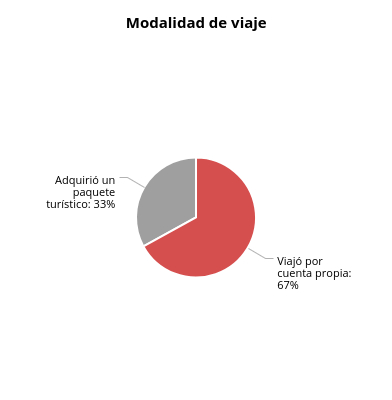
\includegraphics[scale=0.7]{Capitulo2/Figs/modalidad_viaje_extrajero.jpg}
    \caption{Porcentaje de modalidad de viaje de turista extranjero que visita Puno}
    Fuente: \citeA{2017PerfilExtranjero}
    \label{fig:modalidad_viaje_extrajero}
\end{figure}

\begin{figure}[!ht]
    \centering
    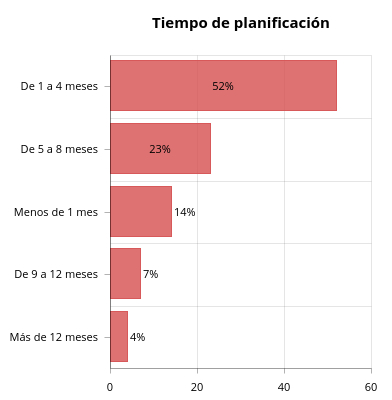
\includegraphics[scale=0.7]{Capitulo2/Figs/tiempo_planificacion_extranjero.jpg}
    \caption{Porcentaje de tiempo de planificación de viaje de turista extranjero que visita Puno}
    Fuente: \citeA{2017PerfilExtranjero}
    \label{fig:tiempo_planificacion_extranjero}
\end{figure}

De acuerdo a otro reporte publicado también publicado por PROMPERU titulado \cite{2017PerfilNacional} se observa que la información que se busca más son las condiciones de las vias de acceso en un 56\%, 49 \%lugares turísticos para visitar, 41\% Costo del trasporte al lugar visitado, 38\% costos de alojamiento y sus características. 

\begin{figure}[!ht]
    \centering
    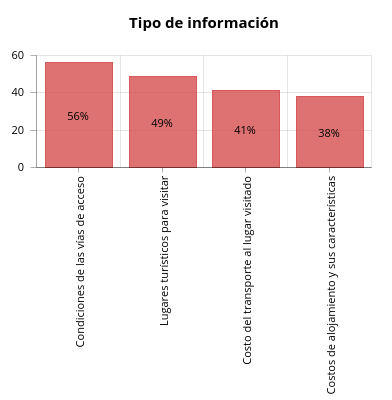
\includegraphics[scale=0.7]{Capitulo2/Figs/tipo_informacion_nacional.jpg}
    \caption{Porcentaje de tipo de información de vacionista nacional que visita Puno}
    Fuente: \citeA{2017PerfilNacional}
    \label{fig:tipo_infomacion_nacional}
\end{figure}

Como podemos ver en la imagen 3 la información que buscan los turistas nacionales son lugares turísticos a visitar en un 82\%, 70\% distancia y rutas de acceso, 66\% restaurantes donde acudir, 24\% costos de alojamiento y sus características, por lo tanto se ve que una solución como la que proponemos ayudará en la toma de decisiones en la planificación de itinerarios en la región Puno.

También al observar que los servicios de agencias de viajes ofrecen son transporte, alojamiento, alimentación, asistencia, etc. Y que los turistas prefieren opciones más personalizadas, en el trabajo que se realizará se considera que se hará un acercamiento a los servicios que brinda las agencias ya que como se puede observar en la imagen 3 las información que buscan lo turistas son relacionados, combinado con la personalización.

La personalización es la palabra clave en el 2018 menciona \citeA{Estadisticas2018-2019} , donde también indica que:
"En 2018, la personalización es el lema al respecto de la experiencia del turista. (Skift, 2018)
Un 57\% de los turistas sienten que las marcas deberían adaptar su información acorde a las preferencias personales o conductas anteriores (Google/Phocuswright, 2017)
Si una marca de turismo adapta su información y experiencia general de la actividad en las preferencias personales o conductas anteriores, un 36\% de los turistas estaría dispuesto a pagar más por sus servicios.(Google/Phocuswright, 2017)"
%Trabajo en el futuro, que pueda cambiar en el momento el itinerario calculando nuevamente el itinerario, de esa manera se provee más flexibilidad.
%Alcance del proyecto
%Limitaciones
%Mencionar como se integrará la aplicaciones de reserva online
\subsection{Social}
Esta investigación apoyará directamente al turista en la toma de decisiones en el diseño de un itinerario detallado para realizar de forma satisfactoria su viaje a la región de Puno, porque se consideran sus preferencias. Y los ciudadanos y los emprendedores de forma indirecta fortaleciendo la valoración cultural, la preservación del medio ambiente y el sentido de identidad nacional. 
\subsection{Económico}
%Con esta investigación se considera que ayudará a que los turistas a minimizar su tiempo en la planificación, también a optimizar el tiempo durante la visita el cual puede ayudar a realizar otras actividades que puedan generarle dinero.

Se ha observado que Puno ha subido en la ultima década en pobreza de acuerdo a una clasificación en el cual Puno se ubicaba antes en el tercer grupo pasando al segundo grupo de departamentos con más pobreza y pobreza extrema según reporte de \citeA{Informe2007-2017}, por ello es importante considerar que con esta investigación al ayudar en que tenga una alternativa que le puede brindar a que tenga una visita mas satisfactoria para que pueda luego recomendar, de esa manera traer a más turistas. Ello ayudará en la reducción de la pobreza como lo menciona \citeA{ElPobreza}. “El turismo, en muchos países en desarrollo y menos adelantados, es la opción de desarrollo económico más viable y sostenible y, en algunos de ellos, la principal fuente de entrada de divisas. Parte de estos ingresos revierte en diferentes grupos de la sociedad y, si el turismo se gestiona centrándose prioritariamente en la atenuación de la pobreza, puede beneficiar directamente a los grupos más pobres mediante el empleo de la población local en empresas turísticas, el suministro de bienes y servicios a los turistas, la gestión de pequeñas empresas y empresas comunitarias, etc., con el consecuente impacto positivo en la reducción de la pobreza”. 
\subsection{Ambiental}
Directamente se considera que ayudará en que se reduzcan el uso de papeles en la guías,etc., al usar la aplicación web, considerado tambien por \citeA{2015PlanPENTUR} como una de las políticas de ambientales en el sector turismo Promover la reducción del consumo de recursos, el reuso, el reciclaje y la ecoeficiencia como estrategias de apoyo al control del deterioro ambiental.  Tambien al utilizar la tecnología para gestionar y limitar la demanda como lo menciona \citeA{InformeTrekkSoft} "Con los sistemas de reserva y venta de entradas, las atracciones populares pueden permitir que los visitantes reserven sus lugares con anticipación, reduciendo el tiempo de espera en las filas y el número de personas que ocupan las calles esperando para entrar."
%TODO: Revisa lo de citar a PERTUR.
\subsection{Ciencia}
Se ha observado que hay escasez de investigaciones relacionadas con el tema de planificación de viajes personalizados en el Perú, de acuerdo a repositorio Repositorio Digital del CONCYTEC llamado ALICIA (Acceso Libre a la Información Científica). Al publicar esta investigación se hará un aporte además de ser local por tratarse de la región de Puno también será un aporte a nivel país.

El problema que se aborda en esta investigación se encuentra dentro de los difíciles que se pueden encontrar la solución y según \citeA{Derivando2017QueYouTube} Estudiar este tipo de problemas es una cuestión muy importe en computación y con muchas aplicaciones.

Ya que la aplicación pretende recolectar información del turista y recolectar información detallada de los atractivos, está podrá ser usado para un posterior análisis para otros usos. Uno de los usos se considera, para una compresión mejor del comportamiento de los turistas para así mejorar los servicios.
%\subsection{Legal}
 %Para generar políticas públicas a través del estado para que puedan ayudar a proteger los atractivos según la ley Nro. 29408 - Ley General de Turismo (2009).
%\subsection{IFE}
%El estudio por los algoritmos, la complejidad computacional que se puede ver que tiene varias aplicaciones y realizar una aplicación que se va a mejorar a través de la retroalimentación que se vaya investigando e implementando. 
\section{Presunción filosófica}
%El avance de la tecnología, Dios
%La inteligencia
%Optimización
%El aporte como un antecedente a la Biblia?
%Presumir? 
%Ejemplo tesis del Dr, Sanchez
